
\section{Протоколы общения дрона и наземной станции}
Рассмотрим подробнее устройство MAVLink.
Формат пакета MAVLink.
Ниже приведен беспроводной формат пакета MAVLink v2 . Представление в памяти может отличаться.

uint8\_t magic;              ///< protocol magic marker
uint8\_t len;                ///< Length of payload
uint8\_t incompat\_flags;     ///< flags that must be understood
uint8\_t compat\_flags;       ///< flags that can be ignored if not understood
uint8\_t seq;                ///< Sequence of packet
uint8\_t sysid;              ///< ID of message sender system/aircraft
uint8\_t compid;             ///< ID of the message sender component
uint8\_t msgid 0:7;          ///< first 8 bits of the ID of the message
uint8\_t msgid 8:15;         ///< middle 8 bits of the ID of the message
uint8\_t msgid 16:23;        ///< last 8 bits of the ID of the message
uint8\_t payload[max 255];   ///< A maximum of 255 payload bytes
uint16\_t checksum;          ///< X.25 CRC
uint8\_t signature[13];      ///< Signature which allows ensuring that the link is tamper-proof (optional)
Формат пакета MAVLink 1 аналогична, но опускает incompat\_flags, compat\_flagsи signature, и имеет только один байт для адреса сообщения. Для получения дополнительной информации см. Сериализация> Формат пакета .

Сериализация
Беспроводной формат MAVLink оптимизирован для систем с ограниченными ресурсами и, следовательно, порядок полей не такой, как в спецификации XML. Беспроводной генератор сортирует все поля сообщения по размеру, uint64\_tсначала с самыми большими полями ( ), а затем с меньшими полями. Сортировка выполняется с использованием стабильного алгоритма сортировки , который гарантирует, что любые поля, которые не нужно переупорядочивать, останутся в том же относительном порядке. Это предотвращает проблемы с выравниванием в системах кодирования / декодирования и позволяет очень эффективно упаковывать / распаковывать.

Для получения дополнительной информации и конкретных исключений см. Сериализация .

Многоадресные потоки и гарантированная доставка
MAVLink создан для гибридных сетей, в которых высокоскоростные потоки данных от источников данных (обычно беспилотных летательных аппаратов) поступают в приемники данных (обычно наземные станции), но смешиваются с передачами, требующими гарантированной доставки. Ключевой вывод состоит в том, что для большинства потоков телеметрии не существует известного или единственного получателя: вместо этого, как правило, бортовой компьютер, наземная станция управления и облачная система нуждаются в одном и том же потоке данных.

С другой стороны, настройка бортовой миссии или изменение конфигурации системы с бортовыми параметрами требует двухточечной связи с гарантированной доставкой. MAVLink достигает очень высокой эффективности за счет использования обоих режимов работы.

Тематический режим (публикация-подписка)
В тематическом режиме протокол не будет выдавать идентификатор целевой системы и компонента для сообщений, чтобы сэкономить пропускную способность канала. Типичными примерами этого режима связи являются все потоки данных автопилота, такие как положение, отношение и т. Д.

Основное преимущество этого многоадресного режима заключается в том, что не создаются дополнительные накладные расходы, и все несколько абонентов могут получать эти данные.

Двухточечный режим
В режиме «точка-точка» MAVLink использует идентификатор цели и целевой компонент. В большинстве случаев, когда используются эти поля, подпротокол также обеспечивает гарантированную доставку (миссии, параметры, команды).

Проверки целостности / Контрольная сумма
MAVLink реализует две проверки целостности: первая проверка целостности пакета во время передачи с использованием контрольной суммы X.25 ( $CRC-16-CCITT$ ). Однако это только гарантирует, что данные не были изменены в ссылке - это не гарантирует согласованности с определением данных. Вторая проверка целостности связана с описанием данных, чтобы убедиться, что два сообщения с одинаковым идентификатором действительно содержат одинаковую информацию. Для этого само определение данных проходит через CRC-16-CCITT, а полученное значение используется для заполнения пакета CRC. Большинство эталонных реализаций хранят эту константу в массиве CRC\_EXTRA .
%
MAVLink — это протокол информационного взаимодействия с беспилотными летательными аппаратами. MAVLink распространяется под LGPL лицензией в виде модуля для python и генератора библиотек под различные языки. 

Протокол описывает информационное взаимодействие между системами, такими как MAV и GCS(Ground control station) — станция наземного управления, а так же их составными частями — компонентами. Базовой сущностью MAVLink является пакет, имеющий следующий формат:

% ~\ref{fig:mavlink}
\begin{figure}[H]
	\centering
	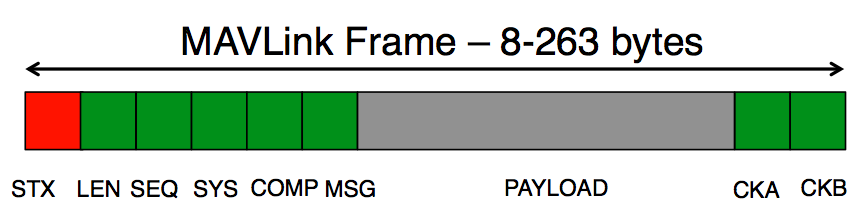
\includegraphics[width=0.5\linewidth]{pics/mavlink}
	\caption{Вращение вокруг оси OZ
	}
	\label{fig:mavlink}
\end{figure}

Первый байт пакета (STX) — это символ начала сообщения: 0xFD для версии v2.0, 0xFE для версии v1.0, 0x55 для версии v0.9. LEN — длинна полезной нагрузки (сообщения). SEQ — содержит счётчик пакета (0-255), который поможет нам выявить потерю сообщения. SYS (System ID) — идентификатор отправляющий системы, а COMP (Component ID) — идентификатор отправляющего компонента. MSG (Message ID) — тип сообщения, от него зависит, какие данные будут лежать в полезной нагрузки пакета. PAYLOAD — полезная нагрузка пакета, сообщение, размером от 0 до 255 байт. Два последних байта пакета — CKA и CKB, нижний и верхний байт, соответственно, содержат контрольную сумму пакета.

Библиотека MAVLink позволяет кодировать и раскодировать пакеты согласно протоколу, но она не регламентирует, какими аппаратными и программными средствами данные будет отправлены — это могут быть TCP/UDP сообщения, обмен через последовательный порт, - все, что обеспечивает двухсторонний обмен. Библиотека обрабатывает входные данные побайтово, добавляя их в буфер и сама собирает из них пакет. Каждая система или компонент, может одновременно обмениваться данными по разным источникам, тогда для каждого источника назначается специальный идентификатор, называемый channel (канал). MAVLink содержит буфер на каждый канал.

\url{https://habr.com/ru/post/312300/}

Канал связи
Протокол MAVLink может быть использован поверх следующих каналов связи:
последовательное соединение (UART, USB и др.);
UDP (Wi-Fi, Ethernet, 3G, LTE);
TCP (Wi-Fi, Ethernet, 3G, LTE).
Сообщение
MAVLink-сообщение это отдельная "порция" данных, передаваемая между устройствами. Отдельное MAVLink-сообщение содержит информацию о состоянии дрона или команду для дрона.

Примеры MAVLink-сообщений:
ATTITUDE, ATTITUDE\_QUATERNION – ориентация квадрокоптера в пространстве;
LOCAL\_POSITION\_NED – локальная позиция квадрокоптера;
GLOBAL\_POSITION\_INT – глобальная позиция квадрокоптера (широта/долгота/высота);
COMMAND\_LONG – команда для квадрокоптера (взлететь, сесть, переключить режим и т. д.).
Полный список MAVLink-сообщений можно посмотреть в документации MAVLink.

Система, компонент системы
Каждое устройство (дрон, базовая станция и т. д.) имеет ID в сети MAVLink. В PX4 MAVLink ID менятся с помощью параметра MAV\_SYS\_ID. Каждое MAVLink сообщение содержит поле с ID системы-отправителя. Кроме того, некоторые сообщения (например, COMMAND\_LONG) содержат также ID системы-получателя.

\url{https://clover.coex.tech/ru/mavlink.html}

\subsection{smthng}

\url{https://dev.px4.io/v1.9.0/en/ros/offboard_control.html}
